\section{Topologia zredukowanego produktu}
\begin{df}
  Niech $M$, $N$ będą przestrzeniami topologicznymi, niech $A$ będzie podzbiorem domkniętym przestrzeni $M$. Definiujemy przestrzeń $(M \times N)_A := (M \setminus A) \times N \cup A$ iloczynu przestrzeni $M$ i $N$ zredukowanego nad $A$ z następującą topologią.
  
  Niech
  \[
    p: (M \times N)_A \rightarrow M
  \]
  będzie odwzorowaniem określonym następująco:
  \begin{enumerate}
    \item $p(m, n) := m$, dla $m \in M \setminus A$
    \item $p(a) := a$, dla $a \in A$
  \end{enumerate}
  
  \begin{figure}[h!]
    \centering
    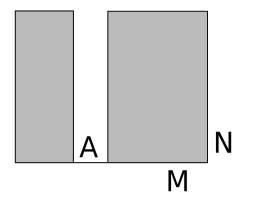
\includegraphics[scale=.5]{img/reduced-product.pdf}
    \caption{Zredukowany produkt $(M\times N)_A$}
  \end{figure}
  
  Topologię na zbiorze $(M \times N)_A$ określamy poprzez bazę złożoną ze zbiorów dwu rodzajów:
  \begin{enumerate}
    \item $U \times V$, gdzie $U \subset M \setminus A$, $U$ otwarty w $M$, $V$ otwarty w $N$
    \item $p^{-1}(U)$, gdzie $U$ jest otwarty w $M$
  \end{enumerate}
  
  Zdefiniujemy również naturalne odwzorowanie $p: M\times N \to (M\times N)_A$, które będziemy nazywać projekcją, następującym wzorem:
  \[
    p(m,n) := \begin{cases}
      m,& m\in A \\
      (m,n),& m\not\in A
    \end{cases}
  \]
\end{df}

\begin{prop} \label{prop:reduced-prod-first-countable}
  Niech $M$, $N$ będą przestrzeniami topologicznymi spełniającymi pierwszy aksjomat przeliczalności, niech $\cl A = A \subset M$. Wówczas $(M\times N)_A$ również spełnia pierwszy aksjomat przeliczalności.
  \begin{proof}
    Jeśli $(m,n) \in (M\setminus A) \times N$, to jako bazę otoczeń punktu $(m,n)$ możemy wziąć $U\times V$, gdzie $U$ i $V$ należą do przeliczalnych baz otoczeń punktów $m$ i $n$ odpowiednio. Jeśli natomiast $a \in A$, to przeliczalną bazę otoczeń punktu $a$ otrzymujemy poprzez wzięcie przeciwobrazu przeliczalnej bazy otoczeń $a$ w $M$ poprzez odwzorowanie $p$ zadające topologię.
  \end{proof}
\end{prop}

Z uwagi na stwierdzenie \ref{prop:reduced-prod-first-countable} w przestrzeni $(M\times N)_A$, gdzie $M$ i $N$ są przestrzeniami metrycznymi a $A$ domkniętym podzbiorem $M$, możemy do badania ciągłości używać zwykłych ciągów.

\begin{lem} \label{lem:reduced-product-continuous}
  Niech $M$, $N$ i $Y$ będą przestrzeniami metrycznymi, $A$ domknięty podzbiór $M$, $n_0 \in N$. Wówczas funkcję $f_0: (M \times N)_A \rightarrow Y$ możemy zareprezentować przez funkcję $f: M \times N \rightarrow Y$ stałą nad $A$, tzn. $N \ni n \rightarrow f(a, n) \in Y$ jest stała przy każdym ustalonym $a \in A$. Funkcje te można wzajemnie odtwarzać wzorami:
  \begin{enumerate}
   \item $f_0(m,n) := f(m,n)$, gdy $(m,n) \in (M \setminus A) \times N$, $f_0(a) := f(a, n_0)$, gdy $a \in A$
   \item $f(m,n) := f_0(p(m,n))$, gdy $(m,n) \in M \times N$,
  \end{enumerate}
  gdzie $p: M\times N \to (M\times N)_A$ jest projekcją.

  
  Co więcej, $f$ reprezentuje funkcję ciągłą $f_0$ wtedy i tylko wtedy gdy $\forall (m_i, n_i)_{i=1}^\infty \in (M \times N)^{\mathbb{N}_1}:$
  \[m_i \rightarrow a \in A \mbox{ pociąga } f(m_i, n_i) \rightarrow f(a, n_1)\]
  
  \begin{proof}
    Niech $(m_i, n_i)_{i=1}^\infty \in (M \times N)^{\mathbb{N}_1}$ i $m_i \rightarrow a \in A$.
    
    Wówczas z definicji topologii na $(M \times N)_A$ zachodzi $p(m_i, n_i) \rightarrow a$. A więc wobec ciągłości $f_0$ otrzymujemy: $f(m_i, n_i) = f_0 p(m_i, n_i) \rightarrow f_0(a) = f(a, x_1)$.
    
    Z drugiej strony, wykażemy ciągłość $f_0$. Funkcja $f_0$ wyraźnie dzieli się na dwa wzory:
    \begin{enumerate}
     \item $f_0|_A(a) = f(a, n_0)$, który to wzór definiuje funkcję ciągłą określoną na domkniętym zbiorze $A$
     \item $f_0|_{(M \setminus A) \times N}(y) = f(y)$, który również ze względu na topologię $(M \times N)_A$ jest wzorem ciągłym, jednak zbiór $(M \setminus A) \times N$ nie musi być domknięty
    \end{enumerate}
    Wystarczy więc sprawdzić przypadek ciągu $p(m_i, n_i) \rightarrow a \in A$, który wykaże, że $f_0|_{\cl{(M \setminus A) \times N}}$ jest funkcją ciągłą, gdyż $\bd((M \setminus A) \times N) = \bd A \subset A$. Ale wówczas z definicji topologii zredukowanego produktu $m_i \rightarrow a \in A$, co z założenia daje $f_0 p(m_i, n_i) = f(m_i, n_i) \rightarrow f(a, x_1) = f_0(a)$, czyli ciągłość $f_0$.
  \end{proof}
\end{lem}

\begin{lem} \label{lem:reduced-product-homeo}
  Niech $U$, $V$ i $Y$ będą przestrzeniami metrycznymi, $A = \cl A \subset U$, niech  $f: U \to V$, homeomorfizm. Wówczas funkcja:
  \[
    h_0: (U \times Y)_A \to (V \times Y)_{f(A)}
  \]
  określona wzorem:
  \[
    \begin{cases}
      h_0(a) := f(a)& a\in A \\
      h_0(u,y) := (f(u), y)& m\not\in A
    \end{cases}
  \]
  jest również homeomorfizmem.
  \begin{proof}
    Zauważmy, że wystarczy sprawdzić ciągłość $h_0$. Istotnie, jeśli $h_0$ będzie ciągłe, to odwrotną do niego funkcję otrzymujemy dokładnie tym samym wzorem z postawieniem $f^{-1}$ za $f$.

    Niech $q: V\times Y \to (V\times Y)_{f(A)}$ będzie projekcją. Wówczas funkcja $h: U\times Y \to (V\times Y)_{f(A)}$ odpowiadająca $h_0$ wygląda następująco:
    \[
      h(u,y) = q(f(u),y)
    \]
    Sprawdzamy więc wymagany w \ref{lem:reduced-product-continuous} warunek. Bierzemy ciąg $(u_i, y_i) \in (U\times Y)^\Ni$. Niech $u_i \to a \in A$. Wówczas mamy:
    \[
      h(u_i,y_i) = q(f(u_i), n_i) \to f(a) = q(f(a),y_1) = h(a,y_1)
    \]
    Zatem $h_0$ jest homeomorfizmem między $(U \times Y)_A$ a $(V \times Y)_{f(A)}$.
  \end{proof}
\end{lem}

\begin{lem} \label{lem:reduced-product-subspace}
  Niech $Y$, $X$ będą przestrzeniami topologicznymi. Niech $F$ będzie domkniętym podzbiorem $Y$. Niech $F_0$ będzie podzbiorem $Y$. Wówczas topologia zredukowanego produktu na $L := ((Y\setminus F_0)\times X)_{F\setminus F_0}$ pokrywa się z topologią indukowaną z $P := (Y\times X)_F$ na $L$.
  
  \begin{proof}
    Widzimy, że zbiór $F\setminus F_0$ jest zbiorem domkniętym w $Y\setminus F_0$ jako ślad zbioru domkniętego $F$ na $Y\setminus F_0$.
    Przypomnijmy, że:
    \begin{align*}
    ((Y\setminus F_0)\times X)_{F\setminus F_0} = ((Y\setminus F_0) \setminus (F\setminus F_0)) &\times X \cup (F\setminus F_0) \\
    = ((Y\setminus F)\setminus F_0) &\times X \cup (F\setminus F_0)
    \end{align*}

    Niech $x \in ((Y\setminus F) \setminus F_0)\times X$. Wówczas otoczenie $x$ w $L$ jest postaci $U\times V$, gdzie $U$ jest zbiorem otwartym w $(Y\setminus F)\setminus F_0$, a $V$ jest zbiorem otwartym w $X$. Zatem $U$ jest śladem pewnego zbioru $\tilde{U}$ otwartego w $Y\setminus F$, tzn. $U = \tilde{U} \cap ((Y\setminus F)\setminus F_0)$. Ale zbiór $\tilde{U}\times V$ jest otoczeniem $x$ w $P$. Co więcej, jeśli $\tilde{U}\times V$ jest otoczeniem $x$ w $P$, to $U\times V$, gdzie $U := \tilde{U}\cap((Y\setminus F)\setminus F_0)$, jest otoczeniem $x$ w $L$.
    
    Niech teraz $x\in F\setminus F_0$. Otoczenia $x$ w $L$ są postaci $(p|_{L})^{-1}(U)$, gdzie $p$ jest odwzorowaniem zadającym topologię na $P$ a zbiór $U$ jest otwarty w $Y\setminus F_0$. Ale wtedy $U$ jest śladem pewnego zbioru $\tilde{U}$ otwartego w $Y$, tzn. $U = \tilde{U}\cap(Y\setminus F_0)$. Ponadto, jeśli $\tilde{U}$ jest otwartym otoczeniem $x$ w $Y$, to $U := \tilde{U}\cap(Y\setminus F_0)$ jest otoczeniem $x$ w $Y\setminus F_0$. Zauważmy, że zachodzi równość:
    \[
      (p|_L)^{-1}(U) = p^{-1}(U) \cap L = p^{-1}(\tilde{U}) \cap L
    \]
    
    Z powyższych rozważań wnioskujemy, że topologia zredukowanego produktu na $L$ pokrywa się z topologią zredukowanego produktu na $P$ indukowaną na $L$.
  \end{proof}
\end{lem}
